\chapter{Introduzione ai linguaggi normali: grammatiche}


\section{Linguaggi (naturali o artificiali)}

La descrizione di un linguaggio avviene su 3 dimensioni:
\begin{itemize}
    \item \textbf{Sintassi}: regole di formazione, ovvero la relazione tra segni
    \item \textbf{Semantica}: attribuzione di significato
    \item \textbf{Pragmatica}: in quale modo frasi corrette e sensate sono usate
    \item \textbf{Implementazione}: come eseguire una frase corretta rispettandone la semantica
\end{itemize}

Partiamo con il descrivere questi elementi

\subsection{Sintassi}

\dfn{sintassi}{La \textbf{sintassi} è la parte della grammatica che studia la struttura delle frasi e il modo in cui le parole si combinano per formare enunciati corretti e significativi}


Si dirama in diversi aspetti: 
\begin{itemize}
    \item \textbf{Aspetto lessicale} che riguarda le parole che si possono usare, quindi:
    \begin{itemize}
        \item descrizione del lessico, intuitivamente i dizionari per i linguaggi naturali assolvono a questo compito
        \item errori dovuti a vocaboli inesistenti
    \end{itemize}
    \item \textbf{Aspetto grammaticale} che si riferisce nel modo in cui è possibile costruire frasi corrette è possibile cotruire con il lessico. Le frasi grammaticalmente corrette possono essere costruite grazie all'uso delle regole grammaticali, che sono in numero finito, mentre il numero di frasi generabili è infinito.
    
    Un errore grammaticale è una frase scorretta, anche se il lessico utilizzato è corretto. Es. "La cane abbaiano"
\end{itemize}

\subsection{Semantica}
\dfn{Semantica}{La \textbf{semantica} è la branca della linguistica che studia il significato delle parole, delle frasi e degli enunciati}

\begin{itemize}
    \item \red{Per il lessico} (quindi lo studio e il significato delle parole) bastano \red{i dizionari}
    \item \red{Per le frasi} è più complicato, \red{devo sapere} infatti:
    \begin{enumerate}
        \item a \red{quale linguaggio appartiene la frase}
        \item su \red{quale linguaggio basarmi per dare significato}
    \end{enumerate}
\end{itemize}

\begin{center}

    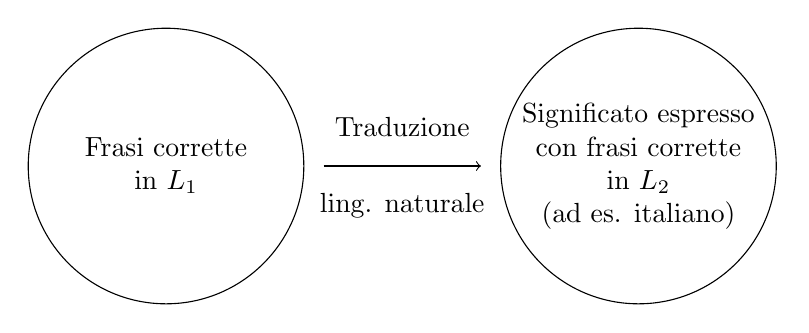
\begin{tikzpicture}
        % Primo cerchio (Frasi corrette in L1)
        \draw (0,0) circle (1.75cm);
        \node at (0,0) {\begin{tabular}{c}
                         Frasi corrette \\ 
                         in \textit{$L_1$}
                         \end{tabular}};
                         
        % Secondo cerchio (Significato espresso con frasi corrette in L2)
        \draw (6,0) circle (1.75cm);
        \node at (6,0) {\begin{tabular}{c}
                         Significato espresso \\ 
                         con frasi corrette \\ 
                         in \textit{$L_2$} \\ 
                         (ad es. italiano)
                         \end{tabular}};
        
        % Freccia tra i due cerchi
        \draw[->] (2,0) -- (4,0);
        \node at (3,0.5) {Traduzione};
        \node at (3,-0.5) {ling. naturale};
    \end{tikzpicture}
\end{center}
\begin{center}
    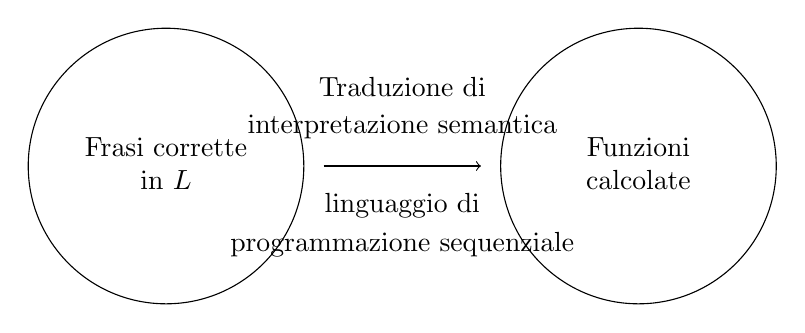
\begin{tikzpicture}
        % Primo cerchio (Frasi corrette in L1)
        \draw (0,0) circle (1.75cm);
        \node at (0,0) {\begin{tabular}{c}
                         Frasi corrette \\ 
                         in \textit{$L$}
                         \end{tabular}};
                         
        % Secondo cerchio (Significato espresso con frasi corrette in L2)
        \draw (6,0) circle (1.75cm);
        \node at (6,0) {\begin{tabular}{c}
                         Funzioni \\ 
                         calcolate \\ 
                         \end{tabular}};
        
        % Freccia tra i due cerchi
        \draw[->] (2,0) -- (4,0);
        \node at (3,1) {Traduzione di};
        \node at (3,0.5) {interpretazione semantica};
        \node at (3,-0.5) {linguaggio di};
        \node at (3,-1) {programmazione sequenziale};
    \end{tikzpicture}
\end{center}

\subsection{Pragmatica}
\dfn{Pregmatica}{
    La \textbf{pragramtica} è un insieme di regole che guidano l'uso e come i contesti influiscono sull'interpretazione di frasi sensate e corrette
}
Ad esempio quando e a chi dare del "tu" o del "lei" quando ci rivolgiamo a delle persone

\subsection{Implementazione}
L'implementazione è \red{l'esecuzione di una frase sintatticamente corretta rispettandone la semantica}

%todo   FINIRE LA FIGURA (ZIO PERA)
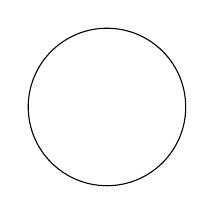
\begin{tikzpicture}
    \draw(0,0) circle (1cm);
    
\end{tikzpicture}

La semantica di $P$, è la funzione $f$ che è pure la semantica del programma compilato $Q$, quindi l'implementazione $Q$ di $P$ preseva la semantica di $P$!

\section{Lessico e frasi di un linguaggio}
Innanzi tutto diamo tre definizioni
\dfn{alfabeto}{
    Un \textbf{alfabeto} è un insieme (tipicamente) finito i cui elementi sono detti simboli 
}
Definire l'alfabeto ci porta alla definizione di lessico:
\dfn{Lessico}{
    Il \textbf{lessico} è un insieme di sequenze finite costituite con caratteri o simboli dell'alfabeto
}
Il quale ci porta alla fenizione di frase:
\dfn{frase}{
    Una \textbf{frase} è un insieme sequenze finite contruite con parole del lessico. 
}
È, quindi, facile notare che \red{il lessico è un alfabeto per le frasi}

Si ci si può ora astrarre e definire un linguaggio formale:
\dfn{linguaggio formale}{
    Un \textbf{linguaggio formale} $L$ su alfabeto $A$ è un sottoinsieme di $A^*$ ($L\subseteq A^*$), dove:
    \[
        A^* = \bigcup_{n \geq 0} A^n \quad \text{ dove } A^0 =\{\epsilon\}       
    \]
    e \[
        A^{n+1}= A\cdot A^n \quad n\geq 0    
    \]
    con $A\cdot A^n = \{aw|a\in A \land w \in A^n\}$
}
Si osservi che \red{$A^*$ è un insieme infinito contabile} dato un ordinamento $ < $ sui simboli di $A$, possiamo elencare tutt le parole come segue:
\begin{enumerate}
    \item elenco la parola vuota $\epsilon$ ($A^0$)
    \item poi elenco le parole di lunghezza 1 ($A^1$) secondo l'ordinamento $ < $
    
    Es. $a,b,c,\dots$
    \item poi elenco le parole in $A^2$ secondo $ < $
    
    Es. $aa, ab, ac, \dots, ba, bb, bc, \dots$
    \item così via
\end{enumerate}

Anche se l'alfabeto $A$ fosse infinito (quindi $A=\{a_0, a_1, \dots\}$) $A^*$ sarebbe ancora contabile, ovvero esisterebbe la possibilità di elencare tutte le possibili parole in $A^*$. Infatti, \red{esiste una biezione tra $A$ e $\mathbb{N}$} e riguardo ai numeri naturali si sa che:
\begin{itemize}
    \item $\mathbb{N}\times \mathbb{N}$ (prodotto cartesiano) è numerabile. La dimostrazione viene fatta attraverso il \textit{dove-tailing}, una tecnica comune per dimostrare la numerabilità di coppie di numeri naturali. Questa dimostrazione introduce la cosìdetta \textbf{funzione di decodifica}
    
    \[
        f^2(x_1,x_2) =\frac{(x_1+x_2)(x_1+x_2+1)}{2} + x_2
    \]
    che presi due numeri in $\mathbb{N}$ completa la seguente tabella ordinando i numeri naturali in "diagonale"
    
    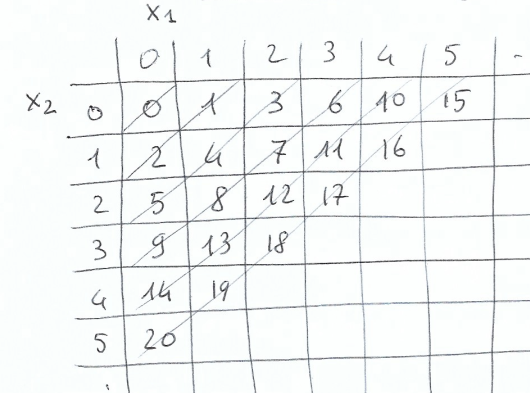
\includegraphics[width=10cm]{funzione_decodifica_tabella.png}

    è pertanto vero, quindi, che
    \[
        f^2:\mathbb{N}\times \mathbb{N}\to \mathbb{N}
    \]
    è biunivoca

    \item $\mathbb{N}^k$ è numerabile. Infatti si può dimostrare attraverso questo algoritmo:
    \[
        f^k(x_1,x_2,\dots,x_k) = \text{ if } (k=2) \text{ then } f^2(x_1,x_2)
        \quad \text{ else } f^2(x_1, f^{k-1}(x_2,\dots,x_k))
    \]
    Ovvero riduce una funzione con $k$ variabili nel dominio ad una serie di funzioni matrioska per ricondurla alla forma $f^2:\mathbb{N}\times\mathbb{N}\rightarrow \mathbb{N}$
    \item $\mathbb{N}^* = \bigcup_{k\geq 0}\mathbb{N}^k$ è numerabile. Infatti:
    \[
        f(x_1,\dots,x_k) = f^2(k,f^k(x_1,\dots, x_k))    
    \]

    
\end{itemize}

\section{Notazioni e definizioni ausiliarie}
Vengono riportate qui alcune definizioni/notazioni
\subsection{Lunghezza}
\dfn{lunghezza}{
    La \textbf{lunghezza} di una parola o stringa è definita per induzione così:
    \begin{itemize}
        \item Caso $|\epsilon|$: $0$
        \item Caso $|aw|$: $1 + |w|$
    \end{itemize}
}
Es: $|abc|=2$ 
\subsection{Concatenazione}
\dfn{Concatenazione}{
    La \textbf{concatenazione} $xy$ tra una stringa $x$ e $y$, è la parola ottenuta giustapponendo $x$ e $y$. Formalmente:
    \[
        w = xy \iff \begin{cases}
            |w|=|x|+|y| \\
            w(j) = x(j) & \text{ per } 1\leq j\leq |x|\\
            w(|x|+j) = x(j) & \text{ per } 1\leq j\leq |y|
        \end{cases}    
    \] 
    Dove $w(j)$ indica il j-esimo simbolo di $w$
}

Questi sono le leggi della concatenazione
\begin{itemize}
    \item Associatività: $x(yz)=(xy)z$
    \item Elemento neutro ($\epsilon$): $x\epsilon = x = \epsilon x$
\end{itemize}

\subsection{Sottostringa}
\dfn{Sottostringa}{
    La stringa $v$ si dive \textbf{sottostringa} di $w \iff \exists x,y \in A^*$ t.c. $w=xvy $ dove $x$ e $y$ possono essere $\epsilon$
}
Si osservi, quindi, che:
\begin{itemize}
    \item Ogni stringa è sottostringa di se stessa
    \item $\epsilon$ è sottostringa di ogni stringa
\end{itemize}

\subsection{Suffisso}
\dfn{suffisso}{
    $v$ si dice \textbf{suffisso} di $w \iff \exists x \in A^x. w=xv$
}
\subsection{Prefisso}
\dfn{prefisso}{
    $v$ si dice \textbf{prefisso} di $w \iff \exists x \in A^x. w=vx$
}
\subsection{Potenza n-esima}
\dfn{potenza n-esima}{
    Si dice \textbf{potenza n-esima} di una stringa $w$ il valore $n\geq 0$ il cui significato è definito per induzione:
    \begin{itemize}
        \item Caso 0: $w^0 = \epsilon$
        \item Caso $n+1$: $w^{n+1}= ww^{n}$
    \end{itemize}
}


\subsection{Linguaggio}
\dfn{linguaggio}{
    Si dice \textbf{linguaggio $L$ su alfabeto $A$} un sottoinsieme $L\subseteq A^*$
}
Vengono riportati qui alcuni esempi
\esempio{
    Se $A=\{a\}$, si possono avere:
    \begin{itemize}
        \item $\emptyset,\{\epsilon\}, \{a,aaa\}$ sono linguaggi finiti
        \item $L_1=\{a^n|\geq 1\}=\{a,aa,aaa,\dots\}=A^*\diagdown \{\epsilon\} $ 
        \item $L_2 =\{a^{2n}|n\geq 0\}=\{\epsilon, aa, aaaa\}$
    \end{itemize}
}
%adssad
\section{Operazione sui linguaggi}
Qui sono elencati le varie operazioni
\subsection{Complemento}
\dfn{complemento}{
    È definito \textbf{complemento} il linguaggio completare ad un linguaggio $L$, ovvero:
    \[
        \overline{L} = \{w\in A^* | w \notin L\} = A^*\diagdown L    
    \]
}
\subsection{Unione e intersezione}
\dfn{unione e intersezione}{
    Ovvi:
    \[
      \begin{array}{l}
            L_1\cup L_2 \{w|w\in L_1 \lor w \in L_2\} \\
            L_1\cap L_2 \{w|w\in L_1 \land w \in L_2\}
      \end{array}
    \]
}

\subsection{Concatenazione}
\dfn{concatenazione}{
    
        È definita \textbf{concatenazione} tale operazione:
        \[
            L_1 \cdot L_2 =\{w_1w_2|w_\in L_1 \land w_2 \in L_2\}
        \]
    
}
Ecco alcuni esempi:
\esempio{
    \begin{itemize}
        \item $L_1 = \{a^n \mid n > 0 \}$ \quad $L_2 = \{b\}$ \\
              $L_1 \cdot L_2 = \{a^n b \mid n > 0\}$
              
        \item $L_1 = \{a^{2n} \mid n > 0 \}$ \quad $L_2 = \{b^m \mid m > 0\}$ \\
              $L_1 \cdot L_2 = \{a^{2n} b^m \mid n, m > 0\}$
              
        \item $L_1 = \{a^m b^n \mid n > 0\}$ \quad $L_2 = \{b^m \mid n > 0\}$ \\
              $L_1 \cdot L_2 = \{a^m b^{n+m} \mid n, m > 0\}$ \\
              \phantom{$L_1 \cdot L_2$} $= \{a^m b^n \mid m \geq n > 0\}$
              
        \item $L_1 = \{a^m \mid m > 1 \}$ \quad $L_2 = \{a^m b^m \mid n > 0 \}$ \\
              $L_1 \cdot L_2 = \{a^{m+n} b^m \mid m > 1, m > 0\}$ \\
              \phantom{$L_1 \cdot L_2$} $= \{a^m b^m \mid m > m > 0\}$
              
        \item $L_1 = \{a b^m \mid n \geq 1\}$ \quad $L_2 = \{a, c\}    \cup \{b^n \mid n \geq 1\}$ \\
              $L_1 \cdot L_2 = \{a b^m a \mid m \geq 1\} \cup \{a b^m c \mid n \geq 1\}$ \\
              \phantom{$L_1 \cdot L_2$} $\cup \{a b^n \mid n \geq 2\}$
              
        \item $A = \{0,1\}$ \\
              $L_1 = \{ w \in A^* \mid w \text{ contiene un numero pari di "0"} \}$ \\
              $L_2 = \{ w \in A^* \mid w = 0y \text{ e } y \in \{1^*\} \}$ \\
              $L_1 \cdot L_2 = \{w \in A^* \mid w \text{ ha un numero dispari di "0"} \}$
    \end{itemize}
}
\subsection{Potenza di un linguaggio}
\dfn{Potenza di un linguaggio}{
    La \textbf{potenza di un linguaggio} viene definita per induzione:
    \begin{itemize}
        \item Caso 0: $L^0 =\{\epsilon\}$
        \item Caso $n+1$: $L\cdot L^n \quad \forall n\geq 0$ 
    \end{itemize}
}

\subsection{Stella di kleene}
\dfn{stella di kleene}{
    Si dice \textbf{stella di kleene}:
    \[
        L^* \bigcup_{n\geq 0} L^n    
    \]
    Oppure 
    \[
        L^+ =   \bigcup_{n\geq 1} L^n   
    \]
    Quest'ultima detta \textbf{chiusura positiva}
}

%asaddsadsa
\section{Definire finitamente un linguaggio}
\subsection{esempio 1: frasi palindrome}
Una frase palindroma è una parola che letta da $sx$ a $dx$ è uguale a se stessa letta da $dx$ a $sx$

Es. "I topi non avevano nipoti"
\begin{itemize}
    \item $A=\{a,b\} \quad L=\{\epsilon, a, b, aa, bb, aba, bab, \dots\}$. Come si nota è piuttosto scomodo
\item Una palindroma può essere: 
        \begin{itemize}
            \item o è la stringa $\epsilon$
            \item oppure a
            \item oppure b
            \item oppure a "palindroma" a
            \item oppure b "palindroma" b
        \end{itemize} 
    \item rappresentazione tramite \textbf{Backus-naur form (BNF)}.
    \[
         \langle P \rangle := \epsilon \mid a\mid b\mid a \langle P \rangle a\mid b \langle P \rangle b   
    \]
    \item  Come \textbf{grammatica}:
    \[
        P\to \epsilon \mid a\mid b\mid aPa\mid bPb    
    \]
    \item definizione ricorsiva in cui:
    \begin{itemize}
        \item $P$ è detto \textit{simbolo non terminale}
        \item $a,b$ sono "simboli terminali"
    \end{itemize}
\end{itemize}
\subsection{Esempio 2}
espressioni aritmetiche formate a partire dalle variabili $a$ e $b$ con gli operatori $\times, +$ e le parantesi $(,)$

Una $expr$ può essere:
\begin{itemize}
    \item \begin{itemize}
        \item la variabile $a$
        \item la variabile $b$
        \item $expr\times expr$
        \item $expr + expr$
        \item ($expr$)
    \end{itemize}
    \item \textbf{bnf}:
      \[
        \langle E \rangle ::= a\mid b\mid \langle E \rangle\times \langle E \rangle \mid \langle E \rangle + \langle E \rangle\mid (\langle E \rangle)
      \]
    \item Grammatica:
    \[
        E\to a\mid b\mid E\times E\mid E+E\mid (E)    
    \]
\end{itemize}

\section{Grammatiche} 
Una grammatica è un insieme di regole che descrivono come le parole e le frasi possono essere combinate per formare espressioni valide. Queste regole determinano la struttura sintattica di un linguaggio, specificando come le unità di base (come le parole o i simboli) si connettono per formare frasi o espressioni più complesse. Ogni grammatica \red{segue lo stesso pattern definito} differenziandosi solo per come sono caratterizzate le produzioni.

Quelle più utili sono le cosiddette grammatiche libere dal contesto (in rapporto tra facilità di analisi ed espressività) 

\dfn{grammatiche libere (dal contesto)}{ \label{dfn: gramLib}
    Una \textbf{grammatica libera} da contesto è una quadrupla $(NT,T,R,S)$ dove:
    \begin{itemize}
        \item \textbf{NT} è un insieme finito di simboli non terminali
        \item $T$ è un insieme finito di simboli terminali
        \item $S\in NT$ è detto simbolo iniziale
        \item $R$ è un insieme finito di produzione (o regole) della forma:
        \[
            V \to w \text{ dove }V\in NT \land w\in (T\cup NT)^*    
        \]
    \end{itemize}
}

Alcuni esempi:
\esempio{
    \[
        G= (\{S\}, \{a,b,+,\times\}, S, R)
    \]
    Con 
    \[
        R=\{S \to a, S \to b, S\to S+S, S\to S\times S\}    
    \]
}

\section{Derivazioni}
\dfn{derivazione immediata}{
    Data $G=(NT, T,R,S)$ libera dal contesto, diciamo che da $v$ si \textbf{deriva immediatamente}  $w$, e lo denotiamo con $v \Rightarrow w$, se:
    \[
        \frac{v =xAy \quad (A\to z )\in R \quad w=xzy}{v\Rightarrow w}    
    \]
    
}
\dfn{derivazione}{
    Diciamo che da $v$ si \textbf{deriva} $w$ (o anche "$v$ si riscrive in $w$"), e lo deontiamo con $v \Rightarrow^* w$, se esiste una sequenza finita (evenutalmente vuota) di derivazione immediate 
    \[
        v \Rightarrow w_0 \Rightarrow w_1 \Rightarrow \dots \Rightarrow w
    \]
    Cioè:
    \[
        \frac{ }{v \Rightarrow^* v} \quad \frac{v\Rightarrow^* w \quad w\Rightarrow z}{v\Rightarrow^* z}    
    \]
    Dove $\Rightarrow^*$ è la chiusa riflessiva e transitiva della relazione $\Rightarrow$
}

\section{Linguaggio Generato}
\dfn{Linguaggio Generato}{
    Il \textbf{linguaggio generato} da una grammatica $<G=(NT, T ,R,S)$ è l'insieme
    \[
        L(G) = \{w\in T^*|S \der w\}
    \]
}

\subsection{Algoritmo di Naif}

Data una grammatica $G$ è opportuno chiedersi come si fa a determinare un linguaggio $L(G)$ e a verificare se $w\in L(G)$. La domanda può essere complessa, tuttavia in casi semplici ci viene in aiuto \textbf{l'algoritmo di Naif} che consiste nel partire da $S$ e provare ad applicare in tutti i modi possibili le produzione (regole) per trovare una derivazione che generi $w$

In certi casi questa verifica è semplice

\esempio{
    \begin{itemize}
        \item 
            Sia $G_3$ con $S\to aSb|ab$

            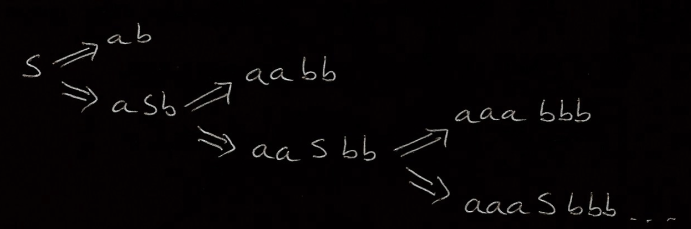
\includegraphics[width=10cm]{alberello.png}
        
            In questo esempio è facile determinare che $L(G_3)=\{a^n b^n|n\geq 1\}$
        \item 
            Sia $G_1 \to aAb \text{ e }A\to aAb\mid \epsilon$ 

            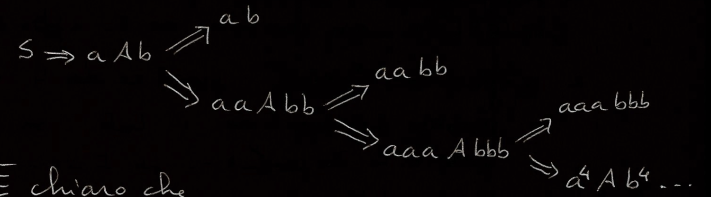
\includegraphics[width=10cm]{alberello_1.png}

            Quindi $L(G_1) = \{a^nb^n\mid n\geq 1\}$
    \end{itemize}

    Si può notare che $G_1 \text{ e } G_3$ sono grammatiche equivalenti perché $L(G_1)=L(G_3)$

    In generale \red{esistono grammatiche diverse che generano lo stesso linguaggio}
    
}

\section{Alberi di derivazione}

Per rappresentare graficamente e semplicemente una certa grammatica esiste uno strumento utilissimo, ovvero l'albero di derivazione

\dfn{albero di derivazione}{ \label{dfn: alberoDer}
    Data una grammatica libera $G= ( NT, T, S, R)$, un albero di derivazione (o di parsing) è un albero ordinato in cui: 
    \begin{itemize}
        \item Ogni nodo è etichettato con un simbolo in $NT \cup \{\epsilon \} \cup T$
        \item la radice è etichettata con $S$
        \item ogni nodo interno è etichettato con un simbolo in $NT$ 
        \item se il nodo $n$
        \begin{itemize}
            \item ha etichetta $A\in NT$ 
            \item i suoi figli sono nell'ordine $m_1,\dots, m_k$ con ,etichetta $x_1,\dots, x_k$ (in $NT\cup T$), allora
            \[
                A \to x_1, \dots , x_k \text{ è una produzione in R }
            \]
        \end{itemize}
        \item se il nodo $n$ ha etichetta $\epsilon$, allora $n$ è una foglia, è figlio unico e, dato $A$ suo padre, $A\to \epsilon$ è una produzione di $R$
        \item se inoltre ogni nodo foglia è etichettato su $T\cup\{\epsilon\}$ è una produzione di $R$
        \item se inoltre ogni nodo foglia è etichettato su $T\cup\{\epsilon\}$, allora l'alberello di derivazione corrisponde ad una derivazione completa
    \end{itemize}
}

Un albero di derivazione, quindi, \red{riassume tante derivazioni diverse ma tutte equivalenti} (ovvero generano lo stesso albero)
\esempio{
    Consideriamo la grammatica 
    \[
        s\to a|b|c|S+S|S \times S
    \]
    Inoltre si consideri la derivazione
    \[
        S \Rightarrow \underbar{S}+S \Rightarrow \underbar{S}\times S + S \Rightarrow a \times \underbar{S}+S \Rightarrow a \times b + \underbar{S} \Rightarrow a\times b + c
    \]
    Allora il suo albero di derivazione è:
    \begin{center}
        
        \begin{tikzpicture}
            \Tree [.S 
                    [.S [.S a ] + [.S b ] ] 
                    * 
                    [.S c ]
                ]
        \end{tikzpicture}
    \end{center}
}
Si osservi inoltre che l'albero di derivazione fornisce informazioni semantiche: "quali operandi per quali operatori" e possono essere riassunti nei cosiddetti \red{alberi sintattici}, tipo
\begin{center}
    
\begin{tikzpicture}
        \Tree [.S 
                [.S [.S a ] + [.S b ] ] 
                $\times$
                [.S c ]
             ]
    \end{tikzpicture}
    e
    
\begin{tikzpicture}
            \Tree [.$\times$ 
                    [
                        .+ 
                        [.a ] 
                        [.b ] 
                    ] 
                    [
                        .c 
                    ] 
                  ]
    \end{tikzpicture}    
\end{center}

        


\teorema{
    Una stringa $w\in T^*$ appartiene a $L(G)$ sse ammette un albero di derivazione completo (le cui foglie, lette da sx a dx diano la stringa $w$) cioè visita in ordine anticipato tralasciando i nonterminali
}


\subsection{Ambiguità}
Per generare una stringa $ w $, una grammatica libera $ G $ puo' avere diversi \textit{alberi di derivazione}, che quindi attribuiscono un significato diverso allo stesso input, vediamo un esempio:
\esempio{ \label{ex: gramAmbi}
    Si consideri la seguente grammatica
    \[
        S\to a|b|c|S+S|S\times S    
    \]
    Si hanno due diverse derivazioni per $a\times b + c$:
    \begin{enumerate}
        \item  $S \Rightarrow \underbar{S}+S \Rightarrow \underbar{S}\times S + S \Rightarrow a \times \underbar{S}+S \Rightarrow a \times b + \underbar{S} \Rightarrow a\times b + c$
        
        con l'albero: 
        \begin{center}
            
\begin{tikzpicture}
                \Tree [.S 
                        [.S [.S a ] $\times$ [.S b ] ] 
                        + 
                        [.S c ]
                    ]
            \end{tikzpicture} 
        \end{center}
        \item $S \Rightarrow \underbar{S}\times S \Rightarrow a \times \underbar{S} \Rightarrow a  \times \underbar{S} + s \Rightarrow a\times b + \underbar{S} \Rightarrow a\times b + c$
        
        Con l'albero:

        \begin{center}
            
\begin{tikzpicture}
            \Tree [.S 
                [.S 
                    [.S b ] 
                    + 
                    [.S c ] 
                ]
                $\times$
                [.S a ] 
            ]
            \end{tikzpicture}
        \end{center}
    \end{enumerate}

}
Nella grammatica dell'esempio \ref{ex: gramAmbi}, la stringa $a\times b + c $ ha più di un albero di derivazione. In questi casi si dice che la grammatica è quindi \red{inutilizzabile per dare semantica a $a\times b + c $} e viene definita \textbf{ambigua}. Bisogna utilizzare grammatiche non ambigue, o manipolare grammatiche ambigue per disambiguarle.
\dfn{Grammatica ambigua}{
Una grammatica libera $G$ è \textbf{ambigua} se $\exists w \in L(G)$ che ammette più alberi di derivazione.
}
E di conseguenza:
\dfn{Linguaggio ambiguo}{
    Un linguaggio $L$ è \textbf{ambiguo} se tutte le grammatiche $G$, tali che $L(G)=L$, sono ambigue
}

Attenzione! Abbiamo detto che una grammatica e' ambigua se, per lo stesso input, ha \textit{alberi} di derivazione diversi, \textbf{NON} \textit{derivazioni} diverse. Questa distinzione e' necessaria perche' due derivazioni possono differire semplicemente nell'ordine in cui sostituisono i nonterminali, generando pero' lo stesso albero di derivazione e quindi attribuendo lo stesso significato all'input. 

\subsubsection{Derivazioni rightmost e leftmost} 
Per poter studiare l'ambiguita' di una grammatica guardando le sue derivazioni, ci e' utile fissare un'unica strategia per decidere quale nonterminale sostitiure ad ogni passaggio di derivazione. Una convenzione semplice e' quella di prendere il nonterminale piu' a sinistra (o a destra) della stringa intermedia di derivazione. Queste due strategie si chiamano derivazioni \textit{leftmost} e \textit{rightmost}:
\dfn{Derivazione leftmost (e rightmost)}{ 
  Sia $ G = (NT, T, R, S) $ una grammatica libera. Diciamo che $ u \Rightarrow_l v $ se $ u = xXy, v = xzy $, dove $ x \in T^*, y \in (T \cup NT)^* $ e $ X \to z \in R $. Se, invece, $ x \in (T \cup NT)^* $ e $ y \in T^* $, allora $ u \Rightarrow_r v $. 

  Quindi, scriviamo $ u \Rightarrow_l v $ quando sostituiamo il nonterminale di $ u $ che si trova piu' a sinistra, e $ u \Rightarrow_r v $ quando sostituiamo quello piu' a destra. Detto cio', una \textbf{derivazione leftmost} e' una derivazione $ u_1 \Rightarrow^*_l u_n $ tale che:
  \[
  u_1 \Rightarrow_l u_2 \Rightarrow_l ... \Rightarrow_l u_n
  \]
  Quindi ad ogni passo sostituiamo il nonterminale piu' a sx (in modo analogo per rightmost).
}\label{dfn: derLeft}
Si puo' dimostrare che, se per una stringa $ w $ esiste un'albero di derivazione per una grammatica $ G $, allora esistono sicuramente derivazioni leftmost e rightmost di $ w $. In piu', possiamo dimostrare che i seguenti numeri sono uguali:
\begin{itemize}
  \item Il numero di derivazioni leftmost di $ w $
  \item Il numero di derivazioni rightmost di $ w $
  \item Il numero di alberi di derivazione distinti di $ w $
\end{itemize}

Detto cio', possiamo utilizzare la definizione di grammatica ambigua per arrivare alla seguente proposizione:
\mprop{Derivazioni leftmost/rightmost e ambiguita'}{
  Data una grammatica libera $ G $, questa' e \textbf{ambigua} sse $ \exists w \in L(G) $ tale che:
  \begin{center}
    $ w $ ha piu' di una derivazione leftmost/rightmost
  \end{center}
}

\subsection{Rimuovere l'ambiguità}
Alcune grammatiche possono essere manipolate di modo da \begin{itemize}
    \item rimuovere l'ambiguità
    \item generare lo stesso linguaggio
\end{itemize}
In altre, invece, ti tieni l'ambiguità (non è possibile rimuoverla (cazzo)). Questa CAZZATA viene spiegata con solo degli esempi:

\esempio{
    Sia $S$ la grammatica
    \[
        S\to a\mid b\mid c\mid S+S\mid S\times S \text{ è ambigua!}       
    \]
    Problemi: \begin{itemize}
        \item Precedenza del * rispetto al + in modo che $a\times b + c$ sia interpretato come:
        \begin{center}
            
\begin{tikzpicture}
                \Tree [.$\times$ 
                        [
                            .+ 
                            [.a ] 
                            [.b ] 
                        ] 
                        [
                            .c 
                        ] 
                      ]
            \end{tikzpicture}  
        \end{center}
        \item associatività del $+$ e del $\times$
        \begin{center}
            \begin{tikzpicture}
            \Tree [.+
                    [
                        .+ 
                        [.a ] 
                        [.b ] 
                    ] 
                    [
                        .c 
                    ] 
                  ]
        \end{tikzpicture}  
        \begin{tikzpicture}
            \Tree [.+
                    [
                        .a
                    ] 
                    [
                        .+ 
                        [.b ] 
                        [.c ] 
                    ] 
                  ]
        \end{tikzpicture}  
    \end{center}
        
        $a+b+c$ ovvero bisogna scegliere l'associatività a dx o sx
        
    \end{itemize}

    Un modo per eliminare questa ambiguità è definire la grammatica così:
    \[
        e\to E+T\mid T \quad T\to A \times T\mid A \quad A \to a\mid b\mid c\mid(E)    
    \]
}
